\documentclass{ximera}

\begin{document}
	\author{Stitz-Zeager}
	\xmtitle{Rational Graphs}{}



\mfpicnumber{1}
\opengraphsfile{RationalGraphs}

\setcounter{footnote}{0}

\label{RationalGraphs}

In Section \ref{IntroRational}, we learned about the types of behaviors to expect from graphs of rational functions: vertical asymptotes, holes in graph, horizontal and slant asymptotes.   Moreover,  Theorems \ref{vavshole}, \ref{hathm} and \ref{sathm} tell us exactly when and where these behaviors will occur.  We used graphing technology extensively in the last section to help us verify results. In this section, we delve more deeply into graphing rational functions with the goal of sketching relatively accurate graphs without the aid of a graphing utility.  Your instructor will ultimately communicate the level of detail expected out of you when it comes to producing graphs of rational functions;  what we provide here is an attempt to glean as much information about the graph as possible given the analytical tools at our disposal.  

  \smallskip

One of the standard tools we will use is the sign diagram which was first introduced in Section \ref{QuadraticFunctions}, and then revisited in Section \ref{RealZeros}. In these sections,  to construct a sign diagram for a function $f$, we first found the zeros of $f$.  The zeros broke  the domain of $f$ into a series of intervals.  We determined the sign of $f(x)$ over the \textit{entire} interval by finding the sign of $f(x)$ for just \textit{one} test value per interval.  The theorem that justified this approach was the Intermediate Value Theorem, Theorem \ref{IVT}, which says that \textit{continuous} functions cannot change their sign between two values unless there is a zero  between those two values. 

This strategy fails in  general with rational functions.  Indeed, the very first  function we studied in Section \ref{IntroRational}, $r(x) = \frac{1}{x}$ changes sign between $x=-1$ and $x=1$, but there is no zero between these two values - instead, the graph changes sign across a vertical asymptote.  We could also well imagine the graph of a rational function having a hole where an $x$-intercept should be.\footnote{Take $f(x) = \frac{x^2}{x}$, for instance.}  With Calculus we can show rational functions are \textbf{continuous on their domains} which means when constructing sign diagrams, we need to choose test values on either side of values excluded from the domain in addition to checking around zeros.\footnote{Since here excluded values are zeros of the denominator, we can think of this as really just generalizing what we already do.}


\phantomsection
\label{rationalsigndiagram}

%% \colorbox{ResultColor}{\bbm

\centerline{\textbf{Steps for Constructing a Sign Diagram for a  Rational Function}} 

\medskip

\hspace{.17in} Suppose $f$ is a rational function. \index{sign diagram ! rational function}

\begin{enumerate}

\item  Place any values excluded from the domain of  $f$ on the number line with an `\textinterrobang' above them.\footnote{ `\textinterrobang' is a nonstandard symbol called the \href{http://en.wikipedia.org/wiki/Interrobang}{\underline{interrobang}}.  \index{interrobang} We use this symbol to convey a sense of surprise, caution and wonderment - an appropriate attitude to take when approaching these points.}   

\item  Find the zeros of $f$ and place them on the number line with the number $0$ above them.

\item  Choose a test value in each of the intervals determined in steps 1 and 2.

\item  Determine and record the sign of $f(x)$ for each test value in step 3.

\end{enumerate}

%% \ebm}

\medskip 

We now present our procedure for graphing rational functions and apply it to a few exhaustive examples.  Please note that we decrease the amount of detail given in the explanations as we move through the examples.  The reader should be able to fill in any details in those steps which we have abbreviated.

\medskip

%% \colorbox{ResultColor}{\bbm

\centerline{\textbf{Steps for Graphing Rational Functions}}

\medskip

\hspace{.17in} Suppose $r$ is a rational function. \index{graph ! rational function}

\begin{enumerate}

\item  Find the domain of $r$.

\item  Reduce $r(x)$ to lowest terms, if applicable.\footnote{This helps us determine limits for the next step.}

\item  Determine the location of any vertical asymptotes or holes in the graph, if they exist. 

\item  Find the axis intercepts, if they exist.

\item  Analyze the end behavior of $r$.  Find the horizontal or slant asymptote, if one exists.

\item  Use a sign diagram and plot additional points, as needed, to sketch the graph.\footnote{It doesn't hurt to check for symmetry at this point, if convenient.}

\end{enumerate}

%% \ebm}

\bigskip

\begin{example}  Sketch a detailed graph of $f(x) = \dfrac{3x}{x^2-4}$.

\smallskip

{\bf Solution.}  We follow the six step procedure outlined above.

\begin{enumerate}

\item  To find the domain, we first find the excluded values.  To that end, we solve  $x^2 - 4 = 0$ and find $x = \pm 2$. Our domain is $\{ x \in \mathbb{R} \, | \,  x \neq \pm 2\}$, or, using interval notation,  $(-\infty, -2) \cup (-2,2) \cup (2,\infty)$.

\item  We check if  $f(x)$ is in lowest terms by factoring: $f(x) = \frac{3x}{(x-2)(x+2)}$.  There are no common factors which means $f(x)$ is already in lowest terms.

\item  Per Theorem \ref{vavshole}, vertical asymptotes and holes in the graph come from values excluded from the domain of $f$.  The two numbers excluded from the domain of $f$ are $x = -2$ and $x=2$ and since  $f(x)$ didn't reduce,  we know $f$ will be unbounded near  $x=-2$ and $x=2$, so we have are vertical asymptotes there.  We can actually go a step further at this point and determine exactly how the graph approaches the asymptote near each of these values. Though not absolutely necessary,\footnote{The sign diagram in step 6 will also determine the behavior near the vertical asymptotes.} it is good practice for those heading off to Calculus.  For the discussion that follows,  we use the factored form of $f(x) = \frac{3x}{(x-2)(x+2)}$.

\begin{itemize}

\item  \textit{The behavior of $y=f(x)$ as $x \rightarrow -2$:}  Suppose $x \rightarrow -2^{-}$.  If we were to build a table of values, we'd use $x$-values a little less than $-2$, say $-2.1$, $-2.01$ and $-2.001$.  While there is no harm in actually building a table like we did in Section \ref{IntroRational}, we want to develop a `number sense' here.  Let's think about each factor in the formula of $f(x)$ as we imagine substituting a number like $x=-2.000001$ into $f(x)$. The quantity $3x$ would be very close to $-6$, the quantity $(x-2)$ would be very close to $-4$, and the factor $(x+2)$ would be very close to $0$.  More specifically, $(x+2)$ would be a little less than $0$, in this case, $-0.000001.$  We will call such a number a `very small $(-)$', `very small' meaning close to zero in absolute value.\footnote{This is the third or fourth time we've used this convention (if you've read the footnotes) so we hope we can just roll with it now.}  So, mentally, as $x \rightarrow -2^{-}$, \[ f(x)   = \dfrac{3x}{(x-2)(x+2)} \approx \dfrac{-6}{(-4)\left( \text{very small $(-)$}\right)} = \dfrac{3}{2 \left( \text{very small $(-)$}\right)} \]  Now, the closer $x$ gets to $-2$, the smaller $(x+2)$ will become, so even though we are multiplying our `very small $(-)$' by $2$, the denominator will continue to get smaller and smaller, and remain negative.  The result is a fraction whose numerator is positive, but whose denominator is very small and negative.  Mentally, \[f(x) \approx \dfrac{3}{2 \left( \text{very small $(-)$}\right)} \approx \dfrac{3}{\text{very small $(-)$}} \approx \text{very big $(-)$}\]  The term `very big $(-)$' means a number with a large absolute value which is negative.\footnote{The actual retail value of $f(-2.000001)$ is approximately $-1,\!500,\!000$.}  What all of this means is that  $\ds{ \lim_{x \rightarrow -2^{-}} f(x) = -\infty}$.    

Now we turn our attention to $x \rightarrow -2^{+}$.  If we imagine substituting something a little larger than $-2$ in for $x$, say $-1.999999$, we mentally estimate \[ f(x) \approx \dfrac{-6}{(-4)\left( \text{very small $(+)$}\right)} = \dfrac{3}{2 \left( \text{very small $(+)$}\right)}  \approx \dfrac{3}{\text{very small $(+)$}} \approx \text{very big $(+)$}\]  We conclude that $\ds{ \lim_{x \rightarrow -2^{+}} f(x) = \infty}$.

\item  \textit{The behavior of $y=f(x)$ as $x \rightarrow 2$:} Consider $x \rightarrow 2^{-}$. We imagine substituting $x = 1.999999$.  Approximating $f(x)$ as we did above, we get \[ f(x) \approx \dfrac{6}{\left( \text{very small $(-)$}\right)(4)} = \dfrac{3}{2 \left( \text{very small $(-)$}\right)}  \approx \dfrac{3}{\text{very small $(-)$}} \approx \text{very big $(-)$}\]  We conclude that $\ds{ \lim_{x \rightarrow 2^{-}} f(x) = -\infty}$.  Similarly, as $x \rightarrow 2^{+}$, we imagine substituting $x = 2.000001$ to get $f(x) \approx \frac{3}{\text{\scriptsize very small $(+)$}} \approx \text{very big (+)}$.  So $\ds{ \lim_{x \rightarrow 2^{+}} f(x) = \infty}$.
\end{itemize}

We interpret this graphically below on the left.


\item  To find the $x$-intercepts of the graph, we set $y=f(x) = 0$.  Solving $ \frac{3x}{(x-2)(x+2)} = 0$ results in $x=0$.  Since $x=0$ is in our domain, $(0,0)$ is the $x$-intercept.   This is also the $y$-intercept,\footnote{Per Exercise \ref{onlyoneyintexercise}, functions can have at most one $y$-intercept. Since $(0,0)$ is on the graph,  it is \textit{the} $y$-intercept.} as we can quickly verify since $f(0) = \frac{3(0)}{0^2-4} = 0$.


\item  Next, we determine the end behavior of the graph of $y=f(x)$.  Since the degree of the numerator is $1$, and the degree of the denominator is $2$, Theorem \ref{hathm} tells us that $y=0$ is the horizontal asymptote.  As with the vertical asymptotes, we can glean more detailed information using `number sense'. For the discussion below, we use the formula $f(x) = \frac{3x}{x^2-4}$. 

\begin{itemize}

\item  \textit{The behavior of $y=f(x)$ as $x \rightarrow -\infty$:}  If we were to make a table of values to discuss the behavior of $f$ as $x \rightarrow -\infty$, we would substitute very `large' negative numbers in for $x$, say for example, $x = \text{$-1$ billion}$.  The numerator $3x$ would then be $-3 \, \text{billion}$, whereas the denominator $x^2-4$ would be $(\text{$-1$ billion})^2 - 4$, which is pretty much the same as  $1(\text{billion})^2$.  Hence, \[f\left(\text{$-1$ billion}\right) \approx \dfrac{-3 \, \text{billion}}{1(\text{billion})^2} \approx - \dfrac{3}{\text{billion}} \approx \text{very small $(-)$} \]

Notice that if we substituted in $x = \text{$-1$ trillion}$, essentially the same kind of cancellation would happen, and we would be left with an even `smaller' negative number.  This not only confirms the fact that as $x \rightarrow -\infty$, $f(x) \rightarrow 0$, it tells us that $f(x) \rightarrow 0^{-}$. In other words, the graph of $y=f(x)$ is a little bit \textit{below} the $x$-axis as we move to the far left.


\item  \textit{The behavior of $y=f(x)$ as $x \rightarrow \infty$:}  On the flip side, we can imagine substituting very large positive numbers in for $x$ and looking at the behavior of $f(x)$.   For example, let $x = \text{$1$ billion}$. Proceeding as before, we get \[f\left(\text{$1$ billion}\right) \approx \dfrac{3 \, \text{billion}}{1(\text{billion})^2} \approx \dfrac{3}{\text{billion}} \approx \text{very small $(+)$} \]  The larger the number we put in, the smaller the positive number we would get out.  In other words, as $x \rightarrow \infty$, $f(x) \rightarrow 0^{+}$, so the graph of $y=f(x)$ is a little bit \emph{above} the $x$-axis as we look toward the far right.  

\end{itemize}

We interpret these findings graphically below on the right.

\begin{center}

\begin{tabular}{cc}

\begin{mfpic}[15]{-4}{4}{-5}{5}

\dashed \polyline{(-2,-4.5), (-2,4.5)}
\dashed \polyline{(2,-4.5), (2,4.5)}
\tlabel[cc](4,-0.5){\scriptsize $x$}
\tlabel[cc](0.5,5){\scriptsize $y$}
\axes
\xmarks{-3 step 1 until 3}
\tiny
\tlpointsep{4pt}
\axislabels {x}{ {$-3\hspace{7pt}$} -3, {$-1\hspace{7pt}$} -1,  {$1$} 1, {$3$} 3}
\normalsize
\penwd{1.25pt}
\arrow \curve{(-2.75,-3),(-2.5,-3.25), (-2.25,-4)}
\arrow \reverse \curve{(-1.75,4),(-1.5,3.25), (-1.25,3)}
\arrow \curve{(1.25,-3), (1.5,-3.25) , (1.75,-4)}
\arrow \curve{(2.75,3),(2.5,3.25), (2.25,4)}
\end{mfpic}

&

\begin{mfpic}[15]{-4.75}{4.75}{-2}{2}
\tlabel[cc](4.75,-0.5){\scriptsize $x$}
\tlabel[cc](0.5,2){\scriptsize $y$}
\axes
\ymarks{-1 step 1 until 1}
\tiny
\tlpointsep{4pt}
\axislabels {y}{{$-1$} -1, {$1$} 1}
\normalsize
\penwd{1.25pt}
\arrow \curve{(2.5,0.85), (3,0.35), (4.25, 0.15)}
\arrow \curve{(-2.5,-0.85), (-3,-0.35), (-4.25, -0.15)}
\end{mfpic} \\

behavior near $x = \pm 2$  & end behavior

\end{tabular}

\end{center}

\item  Lastly, we construct a sign diagram for $f(x)$.  The $x$-values excluded from the domain of $f$ are $x = \pm 2$, and the only zero of $f$ is $x=0$.  Displaying these appropriately on the number line gives us four test intervals, and we choose the test values\footnote{In this particular case, we don't need test values since our analysis of the behavior of $f$ near the vertical asymptotes and our end behavior analysis have given us the signs on each of the test intervals.  In general, however, this won't always be the case, so for demonstration purposes, we continue with our usual construction.} $x=-3$, $x=-1$, $x=1$ and $x=3$.  We find $f(-3)$ is $(-)$, $f(-1)$ is $(+)$, $f(1)$ is $(-)$ and $f(3)$ is $(+)$.  As we begin our sketch, it certainly appears as if the graph could be symmetric about the origin.  Taking a moment to check for symmetry, we find $f(-x) = \frac{3(-x)}{(-x)^2-4} = -\frac{3x}{x^2-4} = -f(x)$.  Hence, $f$ is odd and the graph of $y = f(x)$ is symmetric about the origin. Putting all of our work together, we get the graph below.

\begin{tabular}{m{0.5in}m{2in}m{2.5in}}

&

\begin{mfpic}[10]{-6}{6}{-2}{2}
\arrow \reverse \arrow \polyline{(-6,0),(6,0)}
\xmarks{-3,0,3}
\arrow \polyline{(-4.5,-1.5),(-4.5,-0.5)}
\arrow \polyline{(-1.5,-1.5),(-1.5,-0.5)}
\arrow \polyline{(1.5,-1.5),(1.5,-0.5)}
\arrow \polyline{(4.5,-1.5),(4.5,-0.5)}
\tlpointsep{4pt}
\axislabels {x}{{$-2$} -3, {$0$} 0, {$2$} 3 }
\tlabel[cc](-4.5,1){$(-)$}
\tlabel[cc](-4.5,-2.25){$-3$}
\tlabel[cc](-3,1){\textinterrobang}
\tlabel[cc](-1.5,1){$(+)$}
\tlabel[cc](-1.75,-2.25){$-1$}
\tlabel[cc](0,1){$0$}
\tlabel[cc](1.5,1){$(-)$}
\tlabel[cc](1.5,-2.25){$1$}
\tlabel[cc](3,1){\textinterrobang}
\tlabel[cc](4.5,1){$(+)$}
\tlabel[cc](4.5,-2.25){$3$}
\end{mfpic} 

&

\begin{mfpic}[16]{-6}{6}{-4}{4}

\dashed \polyline{(-2,-4), (-2,4)}
\dashed \polyline{(2,-4), (2,4)}
\tlabel[cc](6,-0.5){\scriptsize $x$}
\tlabel[cc](0.5,4){\scriptsize $y$}
\axes
\xmarks{-5 step 1 until 5}
\ymarks{-3 step 1 until 3}
\tiny
\tlpointsep{4pt}
 \axislabels {x}{ {$-5\hspace{7pt}$} -5, {$-4 \hspace{7pt}$} -4 ,{$-3\hspace{7pt}$} -3, {$-1\hspace{7pt}$} -1,  {$1$} 1, {$3$} 3,  {$4$} 4, {$5$} 5}
\axislabels {y}{ {$-3$} -3, {$-2$} -2,{$-1$} -1, {$1$} 1, {$2$} 2,{$3$} 3}
\normalsize
\penwd{1.25pt}
\arrow \reverse \arrow \function{-6, -2.5, 0.1}{(3*x)/((x**2)-4)}
\arrow \reverse \arrow \function{-1.5, 1.5, 0.1}{(3*x)/((x**2)-4)}
\arrow \reverse \arrow \function{2.5, 6, 0.1}{(3*x)/((x**2)-4)}
\point[4pt]{(0,0)}
\end{mfpic}

\end{tabular}

\end{enumerate}

\qed

\end{example}

Something important to note about the above example is that while $y=0$ is the horizontal asymptote, the graph of $f$ actually crosses the $x$-axis at $(0,0)$.  The myth that graphs of rational functions can't cross their horizontal asymptotes is completely false,\footnote{That's why we called it a MYTH!} as we shall see again in our next example.

\begin{example}  Sketch a detailed graph of $g(t) = \dfrac{2t^2-3t-5}{t^2-t-6}$.

{\bf Solution.}

\begin{enumerate}

\item  To find the values excluded from the domain of $g$, we solve  $t^2-t-6 = 0$ and find $t = -2$ and $t=3$.  Hence, our domain is $\{ t \in \mathbb{R} \, | \, t \neq -2, 3 \}$, or using interval notation: $(-\infty, -2) \cup (-2,3) \cup (3,\infty)$.

\item  To check if $g(t)$ is in lowest terms, we factor:  $g(t) = \frac{(2t-5)(t+1)}{(t-3)(t+2)}$.  There is no cancellation, so $g(t)$ is in lowest terms.

\item  Since $g(t)$ was given to us in lowest terms, we know the graph has vertical asymptotes $t=-2$ and $t=3$.  Keeping in mind $g(t) = \frac{(2t-5)(t+1)}{(t-3)(t+2)}$, we proceed to our analysis near each of these values.

\begin{itemize}

\item  \textit{The behavior of $y=g(t)$ as $t \rightarrow -2$:}  As $t \rightarrow -2^{-}$, we imagine substituting a number a little bit less than $-2$. We have \[g(t) \approx \frac{(-9)(-1)}{(-5)(\text{very small $(-)$})} \approx \frac{9}{\text{very small $(+)$}} \approx \text{very big (+)}\] so  $\ds{ \lim_{t \rightarrow -2^{-}} g(t) = \infty}$. On the flip side, as $t \rightarrow -2^{+}$, we get \[g(t) \approx \frac{9}{\text{ very small $(-)$}} \approx \text{very big $(-)$}\] so  $\ds{ \lim_{t \rightarrow -2^{+}} g(t) = -\infty}$.

\item  \textit{The behavior of $y=g(t)$ as $t \rightarrow 3$:}  As $t \rightarrow 3^{-}$, we imagine substituting a  number just shy  of $3$. We have \[g(t) \approx \frac{(1)(4)}{(\text{ very small $(-)$}) (5)} \approx \frac{4}{\text{very small $(-)$}} \approx \text{very big $(-)$}\] Hence, $\ds{ \lim_{t \rightarrow 3^{-}} g(t) = -\infty}$. As $t \rightarrow 3^{+}$, we get \[g(t) \approx \frac{4}{\text{ very small $(+)$}} \approx \text{very big $(+)$}\] so  $\ds{ \lim_{t \rightarrow 3^{+}} g(t) = \infty}$.

\end{itemize}

We interpret this analysis graphically below on the left.


\item  To find the $t$-intercepts  we set $y = g(t) = 0$.  Using the factored form of $g(t)$ above, we find the zeros to be the solutions of $(2t-5)(t+1)=0$.  We obtain $t = \frac{5}{2}$ and $t=-1$. Since both of these numbers are in the domain of $g$, we have two $t$-intercepts, $\left( \frac{5}{2},0\right)$ and $(-1,0)$.  To find the $y$-intercept, we find $y = g(0) = \frac{5}{6}$, so our $y$-intercept is $\left(0, \frac{5}{6}\right)$.

\item  Since the degrees of the numerator and denominator of $g(t)$ are the same, we know from Theorem \ref{hathm} that we can find the horizontal asymptote of the graph of $g$ by taking the ratio of the leading terms coefficients, $y = \frac{2}{1} = 2$.  However, if we take the time to do a more detailed analysis, we will be able to reveal some `hidden' behavior which would be lost otherwise.  Using long division, we may rewrite $g(t)$ as $g(t) = 2 - \frac{t-7}{t^2-t-6}.$  We focus our attention on the term $\frac{t-7}{t^2-t-6}$.  

\begin{itemize}

\item  \textit{The behavior of $y=g(t)$ as $t \rightarrow -\infty$:} If imagine substituting $t = \text{$-1$ billion}$ into $\frac{t-7}{t^2-t-6}$, we estimate $\frac{t-7}{t^2-t-6} \approx \frac{\text{\scriptsize $-1$ billion}}{1 \text{\scriptsize billion}^2}  = \frac{-1}{\text{\scriptsize billion}} \approx \text{very small $(-)$}$.\footnote{We are once again using the fact that for polynomials, end behavior is determined by the leading term, so in the denominator, the $t^2$ term dominates the $t$ and constant terms.}  Hence, \[g(t) =  2 - \frac{t-7}{t^2-t-6} \approx 2 - \text{very small $(-)$} = 2 + \text{very small $(+)$}\]  Hence, as $t \rightarrow -\infty$, the graph is a little bit \textit{above} the line $y=2$.

\item  \textit{The behavior of $y=g(t)$ as $t \rightarrow \infty$:}  To consider $\frac{t-7}{t^2-t-6}$ as $t \rightarrow \infty$, we imagine substituting $t= \text{$1$ billion}$ and, going through the usual mental routine, find \[\frac{t-7}{t^2-t-6} \approx \text{very small $(+)$}\]  Hence, $g(t) \approx 2 - \ \text{very small $(+)$}$, so the graph is just \textit{below} the line $y=2$ as $t \rightarrow \infty$.

\end{itemize}

We sketch the end behavior below on the right.




\begin{center}

\begin{tabular}{cc}

\begin{mfpic}[15]{-5}{5}{-5}{5}
\dashed \polyline{(-2,-4.5), (-2,4.5)}
\dashed \polyline{(3,-4.5), (3,4.5)}
\tlabel[cc](5,-0.5){\scriptsize $t$}
\tlabel[cc](0.5,5){\scriptsize $y$}
\axes
\xmarks{-4 step 1 until 4}
\tiny
\tlpointsep{4pt}
\axislabels {x}{ {$-3\hspace{7pt}$} -3, {$-1\hspace{7pt}$} -1,  {$1$} 1, {$2$} 2, {$4$} 4}
\normalsize
\penwd{1.25pt}
\arrow \curve{(-2.75,3),(-2.5,3.25), (-2.25,4)}
\arrow \reverse \curve{(-1.75,-4),(-1.5,-3.25), (-1.25,-3)}
\arrow \curve{(2.25,-3), (2.5,-3.25) , (2.75,-4)}
\arrow \curve{(3.75,3),(3.5,3.25), (3.25,4)}
\end{mfpic}

&

\begin{mfpic}[15]{-4.75}{4.75}{-1}{3}
\dashed \polyline{(-4.75,2), (4.75,2)}
\tlabel[cc](4.75,-0.5){\scriptsize $t$}
\tlabel[cc](0.5,3){\scriptsize $y$}
\axes
\ymarks{-1 step 1 until 1}
\tiny
\tlpointsep{4pt}
\axislabels {y}{{$-1$} -1, {$1$} 1}
\normalsize
\penwd{1.25pt}
\arrow \curve{(2.5,1.15), (3,1.65), (4.25, 1.85)}
\arrow \curve{(-2.5,2.85), (-3,2.35), (-4.25, 2.15)}
\end{mfpic} \\

behavior near $t = -2$ and $t = 3$ & end behavior \\

\end{tabular}

\end{center}

\item  Finally we construct our sign diagram.  We place an `\textinterrobang' above $t=-2$ and $t=3$, and a `$0$' above $t = \frac{5}{2}$ and $t=-1$.  Choosing test values in the test intervals gives us $g(t)$ is $(+)$ on the intervals $(-\infty, -2)$, $\left(-1, \frac{5}{2}\right)$ and $(3, \infty)$, and $(-)$ on the intervals $(-2,-1)$ and $\left(\frac{5}{2}, 3\right)$.  As we piece together all of the information, it stands to reason the graph must cross the horizontal asymptote at some point after $t=3$ in order for it to approach $y=2$ from underneath.\footnote{This subtlety would have been missed had we skipped the long division and subsequent end behavior analysis.}   To find where $y = g(t)$ intersects $y = 2$, we solve $g(t) =  2 - \frac{t-7}{t^2-t-6} = 2$ and get $t-7= 0$, or $t=7$.  Note that $t-7$ is the remainder when $2t^2-3t-5$ is divided by $t^2-t-6$, so it makes sense that for $g(t)$ to equal the quotient $2$, the remainder from the division must be $0$.  Sure enough, we find $g(7)=2$.  The location of the $t$-intercepts alone dashes all hope of the function being even or odd (do you see why?) so we skip the symmetry check in this case.

\begin{tabular}{m{0.05in}m{2.5in}m{2.5in}}

&

\begin{mfpic}[10]{-8}{7}{-2}{2}
\arrow \reverse \arrow \polyline{(-8,0),(7,0)}
\xmarks{-5,-2,1,4}
\tlpointsep{4pt}
\axislabels {x}{{$-2$} -5, {$-1$} -2, {$\frac{5}{2}$} 1, {$3$} 4}
\tlabel[cc](-6.5,1){$(+)$}
\tlabel[cc](-5,1){\textinterrobang}
\tlabel[cc](-3.5,1){$(-)$}
\tlabel[cc](-2,1){$0$}
\tlabel[cc](-0.5,1){$(+)$}
\tlabel[cc](1,1){$0$}
\tlabel[cc](2.5,1){$(-)$}
\tlabel[cc](4,1){\textinterrobang}
\tlabel[cc](5.5,1){$(+)$}
\end{mfpic}

& 

\begin{mfpic}[10]{-10}{10}{-5}{9}

\dashed \polyline{(-2,-5), (-2,9)}
\dashed \polyline{(3,-5), (3,9)}
\dashed \polyline{(-10,2), (10,2)}
\tlabel[cc](10,-0.5){\scriptsize $t$}
\tlabel[cc](0.5,9){\scriptsize $y$}
\axes
\xmarks{-9 step 1 until 9}
\ymarks{-4 step 1 until 8}
\tiny
\tlpointsep{4pt}
\axislabels {x}{ {$-9\hspace{7pt}$} -9, {$-8 \hspace{7pt}$} -8 ,{$-7 \hspace{7pt}$} -7, {$-6 \hspace{7pt}$} -6,{$-5\hspace{7pt}$} -5, {$-4 \hspace{7pt}$} -4 ,{$-3\hspace{7pt}$} -3, {$-1\hspace{7pt}$} -1,  {$1$} 1, {$2$} 2,  {$4$} 4, {$5$} 5, {$6$} 6,  {$7$} 7, {$8$} 8, {$9$} 9}
\axislabels {y}{ {$-4$} -4,{$-3$} -3, {$-2$} -2,{$-1$} -1, {$1$} 1, {$3$} 3, {$4$} 4, {$5$} 5, {$6$} 6, {$7$} 7, {$8$} 8}
\normalsize
\penwd{1.25pt}
\arrow \reverse \arrow \function{-9, -2.29, 0.1}{(2*(x**2)-3*x-5)/((x**2)-x-6)}
\arrow \reverse \arrow \function{-1.69, 2.86, 0.1}{(2*(x**2)-3*x-5)/((x**2)-x-6)}
\arrow \reverse \arrow \function{3.12, 9, 0.1}{(2*(x**2)-3*x-5)/((x**2)-x-6)}
\point[4pt]{(-1,0), (2.5,0), (0, 0.83333)}
\end{mfpic}

\end{tabular}

\end{enumerate}

\qed

\end{example}

More can be said about the graph of $y = g(t)$ above.   It stands to reason that $g$ must attain a local  minimum at some point past $t=7$ since the graph of $g$ crosses through $y=2$  at $(2,7)$ but approaches $y=2$ from below as $t \rightarrow \infty$.  Calculus verifies a local minimum at $(13, 1.96)$.  We invite the reader to verify this claim using a graphing utility. 

\begin{example}  Sketch a detailed graph of $h(x) = \dfrac{2x^3+5x^2+4x+1}{x^2+3x+2}$.

{ \bf Solution.}  

\begin{enumerate}

\item   Solving $x^2+3x+2 = 0$ gives $x = -2$ and $x=-1$ as our excluded values.  Hence, the domain is $\{ x \in \mathbb{R} \, | \, x \neq -1, -2 \}$ or, using interval notation,  $(-\infty, -2) \cup (-2, -1) \cup (-1, \infty)$.

\item  To reduce $h(x)$, we need to factor the numerator and denominator.  To factor the numerator, we use the techniques\footnote{Bet you never thought you'd never see \textit{that} stuff again before the Final Exam!} set forth in Section \ref{RealZeros} and get  \[h(x) =  \dfrac{2x^3+5x^2+4x+1}{x^2+3x+2} = \dfrac{(2x+1)(x+1)^2}{(x+2)(x+1)} = \dfrac{ (2x+1) (x+1)^{\cancelto{1}{2}}  }{(x+2)\cancel{(x+1)}} = \dfrac{(2x+1)(x+1)}{x+2} \]

Note we can use this formula for $h(x)$ in our analysis of the graph of $h$ as long as we are not substituting $x=-1$.  To make this exclusion specific, we write $h(x) = \frac{(2x+1)(x+1)}{x+2}$, $x \neq -1$.

\item  Since the factor $(x+2)$ remains in the denominator of $h(x)$ in lowest terms, we expect the graph to have the vertical asymptote $x=-2$.  As for $x=-1$, the factor $(x+1)$ was canceled from the denominator when we reduced $h(x)$, so there will be a hole when $x=-1$.   

\begin{itemize}

\item  \textit{The behavior of $y=h(x)$ as $x \rightarrow -2$:}  As $x \rightarrow -2^{-}$, we imagine substituting a number a little bit less than $-2$. We have $h(x) \approx \frac{(-3)(-1)}{(\text{\scriptsize very small $(-)$})} \approx \frac{3}{(\text{\scriptsize very small $(-)$})}\approx \text{very big $(-)$}$.  Hence,  $\ds{\lim_{x \rightarrow -2^{-}} h(x) = - \infty}$.  On the other side of $-2$, as $x \rightarrow -2^{+}$, we find that $h(x) \approx \frac{3}{\text{\scriptsize very small $(+)$}} \approx \text{very big $(+)$}$, so  $\ds{\lim_{x \rightarrow -2^{+}} h(x) =  \infty}$.

\item  \textit{The behavior of $y=h(x)$ as $x \rightarrow -1$.}    As $x \rightarrow -1$, we have $2x+1 \rightarrow -1$, $x+1 \rightarrow 0$, and $x+2 \rightarrow 1$.  Hence, $\frac{(2x+1)(x+1)}{x+2} \rightarrow \frac{(-1)(0)}{1} = 0$ so $\ds{\lim_{x \rightarrow -1} h(x) = 0}$.  This means we have a hole at $(-1,0)$.  More specifically,\footnote{We'll also see this  when we make the sign diagram later \ldots} we note that as $x \rightarrow -1^{-}$,  $h(x) > 0$ whereas as $x \rightarrow -1^{+}$, $h(x) < 0$. This helps us sketch the graph of $h$ near $(-1,0)$.

\end{itemize}


\item  To find the $x$-intercepts, as usual, we set $h(x) = 0$ and solve.  Solving $\frac{(2x+1)(x+1)}{x+2}=0$ yields $x=-\frac{1}{2}$ and $x=-1$.  The latter isn't in the domain of $h$, in fact, we know there is a hole at $(-1,0)$,  so we exclude it.  Our only $x$-intercept is $\left(-\frac{1}{2}, 0\right)$.  To find the $y$-intercept, we set $x=0$.  Since $0 \neq -1$, we can use the reduced formula for $h(x)$ and we get $h(0) = \frac{1}{2}$ for a $y$-intercept of $\left(0,\frac{1}{2}\right)$.


\item  For end behavior, we note that the degree of the numerator of $h(x)$, $2x^3+5x^2+4x+1$, is $3$ and the degree of the denominator, $x^2+3x+2$, is $2$ so by Theorem \ref{sathm}, the graph of $y = h(x)$ has a slant asymptote.  For $x\rightarrow  -\infty$ or $x \rightarrow \infty$, we are far enough away from $x=-1$ to use the reduced formula, $h(x) = \frac{(2x+1)(x+1)}{x+2}$, $x \neq -1$.  To perform long division, we multiply out the numerator and get $h(x) = \frac{2x^2+3x+1}{x+2}$, $x \neq -1$, and rewrite $h(x) = 2x-1+\frac{3}{x+2}$, $x \neq -1$.  By Theorem \ref{sathm}, the slant asymptote is $y = 2x-1$, and to better see \textit{how} the graph approaches the asymptote, we focus our attention on the term generated from the remainder, $\frac{3}{x+2}$.

\begin{itemize}

\item  \textit{The behavior of $y=h(x)$ as $x \rightarrow -\infty$:} Substituting  $x = \text{$-1$ billion}$ into $\frac{3}{x+2}$, we get the estimate $\frac{3}{\text{\scriptsize $-1$ billion}} \approx \text{very small $(-)$}$.  Hence, $h(x) = 2x-1+\frac{3}{x+2} \approx 2x-1 + \text{very small $(-)$}$.  This means the graph of $y=h(x)$ is a little bit \textit{below} the line $y=2x-1$ as $x \rightarrow -\infty$.

\item  \textit{The behavior of $y=h(x)$ as $x \rightarrow \infty$:}  If $x \rightarrow \infty$, then $\frac{3}{x+2} \approx \text{very small $(+)$}$.  This means $h(x) \approx 2x-1 + \text{very small $(+)$}$, or that the graph of $y=h(x)$ is a little bit \textit{above} the line $y=2x-1$ as $x \rightarrow \infty$.

\end{itemize}

We sketch the end behavior below on the right.
 
 \begin{center}
 
 \begin{tabular}{cc}

\begin{mfpic}[15]{-4}{1}{-5}{5}

\dashed \polyline{(-2,-4.5), (-2,4.5)}
\tlabel[cc](1,-0.5){\scriptsize $x$}
\tlabel[cc](0.5,5){\scriptsize $y$}
\axes
\xmarks{-2,-1}
\tiny
\tlpointsep{4pt}
\axislabels {x}{ {$-3\hspace{7pt}$} -3}
\normalsize
\penwd{1.25pt}
\arrow \curve{(-2.75,-3),(-2.5,-3.25), (-2.25,-4)}
\arrow \reverse \curve{(-1.75,4),(-1.5,3.25), (-1.25,3)}
\curve{(-1.25,0.5), (-1,0), (-0.75,-0.5)}
\pointfillfalse
\point[4pt]{(-1,0)}
\end{mfpic}

&

\begin{mfpic}[15]{-4.75}{4.75}{-4.75}{4.75}

\dashed \function{-1.7,2.7,0.1}{2*x-1}
\tlabel[cc](4.75,-0.5){\scriptsize $x$}
\tlabel[cc](0.5,4.75){\scriptsize $y$}
\axes
\ymarks{-4 step 4 until 1}
\tiny
\tlpointsep{4pt}
\axislabels {y}{{$-4$} -4,{$-3$} -3,{$-2$} -2,{$-1$} -1, {$1$} 1, {$2$} 2, {$3$} 3, {$4$} 4}
\normalsize
\penwd{1.25pt}
\arrow \curve{(-1.25,-4), (-1.5,-4.2), (-1.7, -4.75)}
\arrow \curve{(2.25,4), (2.5,4.2), (2.75, 4.75)}
\end{mfpic} \\

behavior near $x = -2$ and $x=-1$ & end behavior

\end{tabular}

\end{center}

\item  To make our sign diagram, we place an `\textinterrobang' above $x=-2$ and $x=-1$ and a `$0$' above $x=-\frac{1}{2}$.  On our four test intervals, we find $h(x)$ is $(+)$ on $(-2,-1)$ and $\left(-\frac{1}{2}, \infty\right)$ and $h(x)$ is $(-)$ on $(-\infty, -2)$ and $\left(-1,-\frac{1}{2}\right)$.  Putting all of our work together yields the graph below.

\end{enumerate}

\begin{tabular}{m{0.5in}m{2in}m{2.5in}}

&

\begin{mfpic}[10]{-8}{8}{-2}{2}
\arrow \reverse \arrow \polyline{(-8,0),(8,0)}
\xmarks{-4,0,4}
\tlpointsep{6pt}
\axislabels {x}{{$-2 \hspace{9pt}$} -4, {$-1 \hspace{9pt}$} 0, {$-\frac{1}{2} \hspace{9pt}$} 4}
\tlabel[cc](-6,1){$(-)$}
\tlabel[cc](-4,1){\textinterrobang}
\tlabel[cc](-2.25,1){$(+)$}
\tlabel[cc](0,1){\textinterrobang}
\tlabel[cc](2.25,1){$(-)$}
\tlabel[cc](4,1){$0$}
\tlabel[cc](6,1){$(+)$}
\end{mfpic} 

&

\begin{mfpic}[16][8]{-5}{5}{-15}{10}

\dashed \polyline{(-2,-15), (-2,10)}
\dashed \function{-7,5.5,0.1}{2*x-1}
\tlabel[cc](5,-0.5){\scriptsize $x$}
\tlabel[cc](0.5,10){\scriptsize $y$}
\axes
\xmarks{-4 step 1 until 4}
\ymarks{-14 step 1 until 9}
\tiny
\tlpointsep{4pt}
\axislabels {x}{{$-4 \hspace{7pt}$} -4 ,{$-3\hspace{7pt}$} -3, {$-1\hspace{7pt}$} -1,  {$1$} 1,{$2$} 2, {$3$} 3,  {$4$} 4}
\axislabels {y}{ {$-14$} -14, {$-13$} -13,{$-12$} -12,{$-11$} -11, {$-10$} -10,{$-9$} -9,{$-8$} -8, {$-7$} -7,{$-6$} -6,{$-5$} -5, {$-4$} -4,{$-3$} -3, {$-2$} -2,{$-1$} -1, {$1$} 1, {$2$} 2,{$3$} 3, {$4$} 4,{$5$} 5, {$6$} 6,{$7$} 7, {$8$} 8,{$9$} 9}
\normalsize
\penwd{1.25pt}
\arrow \reverse \arrow \function{-6.67, -2.32, 0.1}{(2*(x**2)+3*x+1)/(x+2)}
\arrow \reverse \arrow \function{-1.79, 5.29, 0.1}{(2*(x**2)+3*x+1)/(x+2)}
\point[4pt]{(-0.5,0)}
\pointfillfalse
\point[4pt]{(-1,0)}
\end{mfpic}

\end{tabular}

To find if the graph of $h$ ever crosses the slant asymptote, we solve $h(x) = 2x-1+\frac{3}{x+2}= 2x-1$.  This results in $\frac{3}{x+2} = 0$, which has no solution.\footnote{Alternatively, the remainder after the long division was $r=3$ which is never $0$.} Hence, the graph of $h$ never crosses its slant asymptote.\footnote{But rest assured, some graphs do!}
\qed


\end{example}

Our last graphing example is challenging in that our six step process provides us little information to work with.

\begin{example}   \label{carefulanalysisneeded} Sketch the graph of $r(x) = \dfrac{x^4+1}{x^2+1}$.

\smallskip

{\bf Solution.}

\begin{enumerate}

\item  The denominator $x^2+1$ is never zero which means there are no excluded values.  The domain is $\mathbb{R}$, or using interval notation,  $(-\infty, \infty)$.

\item  With no real zeros in the denominator, $x^2+1$ is an irreducible quadratic.  Our only hope of reducing $r(x)$ is if $x^2+1$ is a factor of $x^4+1$.  Performing long division gives us \[\frac{x^4+1}{x^2+1} = x^2-1+\frac{2}{x^2+1}\] The remainder is not zero so $r(x)$ is already reduced.

\item Since there are no numbers excluded from the domain of $r$, there are no vertical asymptotes or holes in the graph of $r$.

\item  To find the $x$-intercept, we'd set $r(x) = 0$.  Since there are no real solutions to $x^4+1=0$, we have no $x$-intercepts.  Since $r(0) = 1$, we do get $(0,1)$ as the $y$-intercept.

\item  For end behavior, we note that since the degree of the numerator is exactly \textit{two} more than the degree of the denominator, neither Theorems \ref{hathm} nor \ref{sathm} apply.\footnote{This won't stop us from giving it the old community college try, however!} We know from our attempt to reduce $r(x)$ that we can rewrite $r(x) = x^2-1+\frac{2}{x^2+1}$, so we focus our attention on the term corresponding to the remainder, $\frac{2}{x^2+1}$  It should be clear that as $x \rightarrow - \infty$ or $x \rightarrow \infty$, $\frac{2}{x^2+1} \approx \text{very small $(+)$}$, which means $r(x) \approx x^2-1 + \text{very small $(+)$}$.  So the graph $y=r(x)$ is a little bit \textit{above} the graph of the parabola $y=x^2-1$ as $x \rightarrow  -\infty$ and $x \rightarrow \infty$. 


\item  There isn't much work to do for a sign diagram for $r(x)$, since its domain is all real numbers and it has no zeros.  Our sole test interval is $(-\infty, \infty)$, and since we know $r(0) = 1$, we conclude $r(x)$ is $(+)$ for all real numbers.   We check for symmetry, and find $r(-x) = \frac{(-x)^4+1}{(-x)^2+1} = \frac{x^4+1}{x^2+1} = r(x)$, so $r$ is even and, hence, the graph is symmetric about the $y$-axis.  It may be tempting at this point to call it quits, reach for a graphing utility, or ask someone who knows Calculus.\footnote{This is exactly what the authors did in the Third Edition. Special thanks go to Erik Boczko from Ohio University for showing us that, in fact, we could do more with this example algeraically.}  It turns out, we can do a little bit better.  Recall from Section \ref{MonomialFunctions}, that when $|x| <1$ but $x \neq 0$, $x^4 < x^2$, hence $x^4+1 < x^2+1$.  This means for $-1<x<0$ and $0<x<1$, $r(x) = \frac{x^4+1}{x^2+1} < 1$. Since we know $r(0) = 1$, this means the graph of $y = r(x)$ must fall to either side before heading off to $\infty$.  This means $(0,1)$ is a local maximum and, moreover, there are at least two local minimums, at least one on either side of $(0,1)$.  We invite the reader to confirm this using a graphing utility. 



\end{enumerate}

\begin{center}

\begin{tabular}{cc}

\begin{mfpic}[15]{-3}{3}{-2}{6}
\dashed \function{-2.5,2.5,0.1}{x**2-1}
\axes
\ymarks{-1,1,2,3,4,5}
\tiny
\tlpointsep{4pt}
\axislabels {y}{ {$1$} 1, {$2$} 2,{$3$} 3, {$4$} 4,{$5$} 5}
\normalsize 
\penwd{1.25pt}
\arrow \curve{(-2,4), (-2.25,4.5), (-2.5,6)}
\arrow \curve{(2,4), (2.25,4.5), (2.5,6)}
\tlabel[cc](3,-0.5){\scriptsize $x$}
\tlabel[cc](0.5,6){\scriptsize $y$}
\end{mfpic}

&

\begin{mfpic}[15]{-4}{4}{-2}{6}
\tlabel[cc](4,-0.5){\scriptsize $x$}
\tlabel[cc](0.5,6){\scriptsize $y$}
\axes
\xmarks{-3 step 1 until 3}
\ymarks{-1 step 1 until 5}
\tiny
\tlpointsep{4pt}
\axislabels {x}{{$-3\hspace{7pt}$} -3, {$-1\hspace{7pt}$} -1,  {$1$} 1,{$2$} 2, {$3$} 3}
\axislabels {y}{ {$1$} 1, {$2$} 2,{$3$} 3, {$4$} 4,{$5$} 5}
\normalsize
\penwd{1.25pt}
\arrow \reverse \arrow \function{-2.5, 2.5, 0.1}{(x**4+1)/(x**2+1)}
\point[4pt]{(0,1)}
\end{mfpic} \\

end behavior & sketch of $y = r(x)$

\end{tabular}

\end{center}


\qed
\end{example}


Our last example turns the tables and invites us to write formulas for rational functions given their graphs.

\begin{example} \label{rationalfromgraph}  Write formulas for rational functions $r(x)$ and $F(x)$ given their graphs below:

\begin{center}

\begin{tabular}{cc}

\begin{mfpic}[15][10]{-4}{6}{-5}{10}
\axes
\dashed \polyline{(-4,3), (6,3)}
\dashed \polyline{(1, -5), (1,10)}
\xmarks{-3 step 1 until 5}
\ymarks{-4 step 1 until 9}
\scriptsize
\tlabel[cc](6, -0.5){$x$}
\tlabel[cc](0.5, 10){$y$}
\tlabel[cc](-1.25, 5){$(0,5)$}
\tlabel[cc](2.5, -1){$\left(\frac{5}{3}, 0 \right)$}
\gclear \tlabelrect(0, -4){$x=1$}
\tlabel[cc](4,3.5){$y=3$}
\normalsize
\penwd{1.25pt}
\arrow \reverse \arrow \function{-4,0.7,0.1}{3-2/(x-1)}
\arrow \reverse \arrow \function{1.25,6,0.1}{3-2/(x-1)}
\point[4pt]{(0,5), (1.667,0)}
\tcaption{\scriptsize $y=r(x)$}
\end{mfpic}

\begin{mfpic}[15][10]{-4}{6}{-5}{10}
\axes
\dashed \polyline{(-4,3), (6,3)}
\dashed \polyline{(1, -5), (1,10)}
\xmarks{-3 step 1 until 5}
\ymarks{-4 step 1 until 9}
\scriptsize
\tlabel[cc](6, -0.5){$x$}
\tlabel[cc](0.5, 10){$y$}
\tlabel[cc](-1.25, 5){$(0,5)$}
\tlabel[cc](2.5, -1){$\left(\frac{5}{3}, 0 \right)$}
\gclear \tlabelrect(0, -4){$x=1$}
\tlabel[cc](4,3.5){$y=3$}
\normalsize
\penwd{1.25pt}
\arrow \reverse \arrow \function{-4,0.7,0.1}{3-2/(x-1)}
\arrow \reverse \arrow \function{1.25,6,0.1}{3-2/(x-1)}
\point[4pt]{(0,5)}
\pointfillfalse
\point[4pt]{(1.667,0)}
\tcaption{\scriptsize $y=F(x)$}
\end{mfpic}

\end{tabular}

\end{center}

{\bf Solution.}  The good news is the graph of $r$ closely resembles the graph of $F$, so once we know an expression for $r(x)$, we should be able to modify it to obtain $F(x)$.    We are told $r$ is a rational function, so we know there are polynomial functions $p$ and $q$ so that $r(x) = \frac{p(x)}{q(x)}$.  We know from Theorem \ref{complexfactorization}  that we can factor $p(x)$ and $q(x)$ completely in terms of their leading coefficients and their zeros.  For simplicity's sake, we assume neither $p$ nor $q$ has any non-real zeros.  

We focus our attention first on finding an expression for $p(x)$.  When finding the $x$-intercepts, we look for the zeros of $r$ by solving $r(x) = \frac{p(x)}{q(x)} = 0$.  This equation quickly reduces to solving $p(x) =0$.  Since  $\left(\frac{5}{3}, 0 \right)$ is an $x$-intercept of the graph, we know $x = \frac{5}{3}$ is a zero of $r$, and, hence, a zero of $p$.  Since we are shown no other $x$-intercepts, we assume $r$, hence $p$ have no other real zeros (and no non-real zeros by our assumption.)  Theorem \ref{complexfactorization}  gives  $p(x) = a\left(x - \frac{5}{3}\right)^m$ where $a$ is the leading coefficient of $p(x)$ and $m$ is the multiplicity of the zero $x = \frac{5}{3}$.  Since the graph of $y = r(x)$ crosses through the $x$-axis in what appears to be a fairly linear fashion at  $\left(\frac{5}{3}, 0 \right)$, it seems reasonable to set $m=1$.  Hence, $p(x) = a \left(x - \frac{5}{3}\right)$.

Next, we focus our attention on finding $q(x)$.  Per Theorem \ref{vavshole}, the vertical asymptote  $x=1$ comes from a factor of $(x-1)$ in the denominator of $r(x)$.  This means $(x-1)$ is a factor of $q(x)$.  Since there are no other vertical asymptotes or holes in the graph, $x=1$ is the only real zero, hence (per our assumption) only zero of $q$.  At this point, we have $q(x) = b(x-1)^m$ where $b$ is the leading coefficient of $q(x)$ and $m$ is the multiplicity of the zero $x=1$.  Since the graph of  $r$ has the \textit{horizontal} asymptote $y = 3$,Theorem \ref{ha} tells us two  things:  first,  degree of $q$ must match the degree of $p$; second, the ratio $\frac{a}{b} = 3$.   Hence, the degree of $q$ is $1$ so that: 

\[ \begin{array}{rcl}

r(x) & = & \dfrac{a \left(x - \frac{5}{3}\right)}{b(x-1)} \\
       & = & \dfrac{a}{b} \left(\dfrac{x - \frac{5}{3}}{x-1}\right) \\
        & = & 3  \left(\dfrac{x - \frac{5}{3}}{x-1}\right) \\
        & = & \dfrac{3x-5}{x-1}. \end{array} \]

We have yet to use the $y$-intercept, $(0,5)$.  In this case, we use it as a partial check:  $r(0) = \frac{3(0)-5}{0-1} = 5$, as required.  We can sketch $y=r(x)$ by hand, or with a graphing utility, to give a better check of our work.

Now it is time to find a formula for $F(x)$.  The graphs of $r$ and $F$ look identical except the graph has a hole in the graph at $\left(\frac{5}{3}, 0 \right)$ instead of an $x$-intercept.  Theorem \ref{vavshole} tells us this happens because a factor of $\left(x - \frac{5}{3} \right)$ cancels from the denominator when the formula for $F(x)$ is reduced.  Hence, we reverse this process and multiply the numerator and denominator of our expression for $r(x)$ by $\left(x - \frac{5}{3} \right)$:

\[ \begin{array}{rclr}

F(x) & = &  r(x) \cdot \dfrac{\left(x - \frac{5}{3} \right)}{\left(x - \frac{5}{3} \right)} & \\
       & = &  \dfrac{3x-5}{x-1} \cdot \dfrac{\left(x - \frac{5}{3} \right)}{\left(x - \frac{5}{3} \right)} & \\
       & = & \dfrac{3x^2-10x+\frac{25}{3}}{x^2 - \frac{8}{3} x + \frac{5}{3}} & \text{expand}\\
       & = & \dfrac{9x^2-30x+25}{3x^2-8x+5} & \text{multiply by $1 = \frac{3}{3}$ to reduce the complex fraction.}\\ \end{array} \]

Again, we can check our answer by applying the six step method to this function or, for a quick verification, we can use a graphing utility.\footnote{Be warned, however, a graphing utility may not show the hole at  $\left(\frac{5}{3}, 0 \right)$.} \qed
 

\end{example}

Another way to approach Example \ref{rationalfromgraph} is to take a cue from Theorem \ref{linearlaurentlgraphs}.  The graph of $y=r(x)$ certainly \textit{appears} to be the result of moving around the graph of $f(x) = \frac{1}{x}$.  To that end, suppose $r(x) = \frac{a}{x-k} + k$.  Since the vertical asymptote is $x=1$ and the horizontal asymptote is $y=3$, we get $h=1$ and $k=3$.  At this point, we have $r(x) = \frac{a}{x-1}+3$.  We can determine $a$ by using the $y$-intercept, $(0,5)$:  $r(0) =5$ gives us $-a+3 = 5$ so $a = -2$.  Hence, $r(x) = \frac{-2}{x-1}+3$.  At this point we could check the $x$-intercept  $\left(\frac{5}{3}, 0 \right)$ is on the graph, check our answer using a graphing utility, or even better, get common denominators and write $r(x)$ as a single rational expression to compare with our answer in the above example.  

As usual, the authors offer no apologies for what may be construed as `pedantry' in this section.  We feel that the detail presented in this section is necessary to obtain a firm grasp of the concepts presented here and it also serves as an introduction to the methods employed in Calculus. In the end,  your instructor will decide how much, if any, of the kinds of details presented here are `mission critical' to your understanding of Precalculus. Without further delay, we present you with this section's Exercises.

\newpage

\subsection{Exercises}

%% SKIPPED %% \documentclass{ximera}

\begin{document}
	\author{Stitz-Zeager}
	\xmtitle{Exercises for Rational Graphs}{}

\mfpicnumber{1} \opengraphsfile{ExercisesforRationalGraphs} % mfpic settings added 

Suppose $r$ is a rational function.  You can graph the function $r$ using the following six-step procedure:

\begin{enumerate}

\item  Find the domain of $r$.

\item  Reduce $r(x)$ to lowest terms, if applicable.\footnote{This helps us determine limits for the next step.}

\item  Determine the location of any vertical asymptotes or holes in the graph, if they exist. 

\item  Find the axis intercepts, if they exist.

\item  Analyze the end behavior of $r$.  Find the horizontal or slant asymptote, if one exists.

\item  Use a sign diagram and plot additional points, as needed, to sketch the graph.\footnote{It doesn't hurt to check for symmetry at this point, if convenient.}

\end{enumerate}

\begin{problem}\label{sixstepfirst}
Use the six-step procedure
to graph the rational function.  Be sure to draw any asymptotes as dashed lines.

$f(x) = \dfrac{4}{x + 2}$

\begin{solution}
\[
\graph[xmin=-7, xmax=5, ymin=-5, ymax=5]{\frac{4}{x+2};x=-2}
\]
\end{solution}
\end{problem}

\begin{problem}
Use the six-step procedure
to graph the rational function.  Be sure to draw any asymptotes as dashed lines.

$f(x) = 5x(6-2x)^{-1}$ 
\end{problem}  

\begin{problem}
Use the six-step procedure
to graph the rational function.  Be sure to draw any asymptotes as dashed lines.

$g(t) = t^{-2}$
\end{problem} 

\begin{problem}
Use the six-step procedure
to graph the rational function.  Be sure to draw any asymptotes as dashed lines.

$g(t) = \dfrac{1}{t^{2} + t - 12}$
\end{problem}

\begin{problem}
Use the six-step procedure
to graph the rational function.  Be sure to draw any asymptotes as dashed lines.

$r(z) = \dfrac{2z - 1}{-2z^{2} - 5z + 3}$
\end{problem} 

\begin{problem}
Use the six-step procedure
to graph the rational function.  Be sure to draw any asymptotes as dashed lines.

$r(z) = \dfrac{z}{z^{2} + z - 12}$
\end{problem}  

\begin{problem}
Use the six-step procedure
to graph the rational function.  Be sure to draw any asymptotes as dashed lines.

$f(x) = 4x(x^2+4)^{-1}$
\end{problem} 

\begin{problem}
Use the six-step procedure
to graph the rational function.  Be sure to draw any asymptotes as dashed lines.

$f(x) = 4x(x^2-4)^{-1}$
\end{problem} 

\begin{problem}
Use the six-step procedure
to graph the rational function.  Be sure to draw any asymptotes as dashed lines.

$g(t) = \dfrac{t^2-t-12}{t^2+t-6}$
\end{problem} 

\begin{problem}
Use the six-step procedure
to graph the rational function.  Be sure to draw any asymptotes as dashed lines.

$g(t) = 3- \dfrac{5t-25}{t^2-9}$
\end{problem} 

\begin{problem}
Use the six-step procedure
to graph the rational function.  Be sure to draw any asymptotes as dashed lines.

$r(z) = \dfrac{z^2-z-6}{z+1}$
\end{problem}  

\begin{problem}
Use the six-step procedure
to graph the rational function.  Be sure to draw any asymptotes as dashed lines.

$r(z) =-z-2+\dfrac{6}{3-z}$
\end{problem} 

\begin{problem}
Use the six-step procedure
to graph the rational function.  Be sure to draw any asymptotes as dashed lines.

$f(x) = \dfrac{x^3+2x^2+x}{x^2-x-2}$
\end{problem}  

\begin{problem}
Use the six-step procedure
to graph the rational function.  Be sure to draw any asymptotes as dashed lines.

$f(x) = \dfrac{5x}{9-x^2} - x$
\end{problem}   

\begin{problem}
Use the six-step procedure
to graph the rational function.  Be sure to draw any asymptotes as dashed lines.

$g(t) =\dfrac{1}{2}t-1 + \dfrac{t+1}{t^2+1}$
\end{problem} 

\begin{problem}\label{sixsteplast}
Use the six-step procedure
to graph the rational function.  Be sure to draw any asymptotes as dashed lines.\footnote{Once you've done the six-step procedure, use a graphing utility to graph this function on the window $[0, 12] \times [0, 0.25]$ \ldots}

$g(t) = \dfrac{t^{2} - 2t + 1}{t^{3} + t^{2} - 2t}$ 
\end{problem} 

\begin{problem}\label{rationalfromgraphfirst}
Find a possible formula for the function whose graph is given.
$y = f(x)$

\begin{tikzpicture}
  \begin{axis}[
    axis lines=middle,
    xmin=-2, xmax=6,
    ymin=-4, ymax=4,
    xtick={-1,0,1,2,3,4,5},
    xticklabels={$-1$,$0$,$1$,$2$,$3$,$4$,$5$},
    ytick={-3,-2,-1,1,2,3},
    yticklabels={$-3$,$-2$,$-1$,$1$,$2$,$3$},
    axis line style={->},
    width=11cm, height=8cm,
    clip=false
  ]
    % Axis labels
    \node at (axis cs:6,-0.5) {\scriptsize $x$};
    \node at (axis cs:0.5,4) {\scriptsize $y$};

    % Vertical asymptote
    \addplot[dashed] coordinates {(2,-4) (2,4)};

    % Function pieces (avoiding vertical asymptote at x=2)
    \addplot[domain=-2:1.75, samples=200, thick, ->] {1/(x-2)};
    \addplot[domain=2.25:6, samples=200, thick, ->] {1/(x-2)};

    % Points
    \addplot[only marks, mark=*] coordinates {(1,-1) (3,1)};

    % Point labels
    \node at (axis cs:3.75,1.25) {\scriptsize $(3,1)$};
    \node at (axis cs:0.5,-1.5) {\scriptsize $(1,-1)$};

    % Caption below
    \node[below] at (rel axis cs:0.5,0) 
      {\scriptsize Vertical asymptote: $x=2$};
  \end{axis}
\end{tikzpicture}
\end{problem}

\begin{problem}
Find a possible formula for the function whose graph is given.
$y = F(x)$

\begin{tikzpicture}
  \begin{axis}[
    axis lines=middle,
    xmin=-2, xmax=6,
    ymin=-4, ymax=4,
    xtick={-1,0,1,2,3,4,5},
    xticklabels={$-1$,$0$,$1$,$2$,$3$,$4$,$5$},
    ytick={-3,-2,-1,1,2,3},
    yticklabels={$-3$,$-2$,$-1$,$1$,$2$,$3$},
    axis line style={->},
    width=11cm, height=8cm,
    clip=false
  ]
    % Axis labels
    \node at (axis cs:6,-0.5) {\scriptsize $x$};
    \node at (axis cs:0.5,4) {\scriptsize $y$};

    % Vertical asymptote
    \addplot[dashed] coordinates {(2,-4) (2,4)};

    % Function pieces (avoiding asymptote at x=2)
    \addplot[domain=-2:1.75, samples=200, thick, ->] {1/(x-2)};
    \addplot[domain=2.25:6, samples=200, thick, ->] {1/(x-2)};

    % Filled point
    \addplot[only marks, mark=*] coordinates {(1,-1)};
    \node at (axis cs:0.5,-1.5) {\scriptsize $(1,-1)$};

    % Open circle (hole)
    \addplot[only marks, mark=o, mark size=2pt, thick] coordinates {(3,1)};
    \node at (axis cs:4.25,1.25) {\scriptsize hole at $(3,1)$};

    % Caption
    \node[below] at (rel axis cs:0.5,0) 
      {\scriptsize Vertical asymptote: $x=2$};
  \end{axis}
\end{tikzpicture}

\end{problem}

\begin{problem}
Find a possible formula for the function whose graph is given.
$y = g(t)$

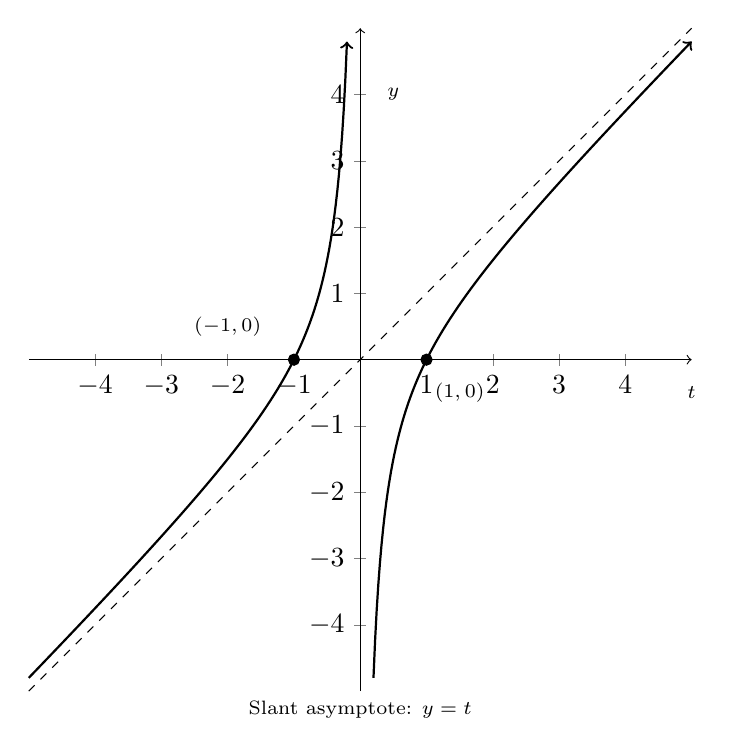
\begin{tikzpicture}
  \begin{axis}[
    axis lines=middle,
    xmin=-5, xmax=5,
    ymin=-5, ymax=5,
    xtick={-4,-3,-2,-1,1,2,3,4},
    xticklabels={$-4$,$-3$,$-2$,$-1$,$1$,$2$,$3$,$4$},
    ytick={-4,-3,-2,-1,1,2,3,4},
    yticklabels={$-4$,$-3$,$-2$,$-1$,$1$,$2$,$3$,$4$},
    axis line style={->},
    width=10cm, height=10cm,
    clip=false
  ]
    % Axis labels
    \node at (axis cs:5,-0.5) {\scriptsize $t$};
    \node at (axis cs:0.5,4) {\scriptsize $y$};

    % Slant asymptote y = t
    \addplot[dashed, domain=-5:5] {x};

    % Function pieces (avoiding asymptote at x=0)
    \addplot[domain=-5:-0.2, samples=200, thick, ->] {x - 1/x};
    \addplot[domain=0.2:5, samples=200, thick, ->] {x - 1/x};

    % Points
    \addplot[only marks, mark=*] coordinates {(-1,0) (1,0)};
    \node at (axis cs:-2,0.5) {\scriptsize $(-1,0)$};
    \node at (axis cs:1.5,-0.5) {\scriptsize $(1,0)$};

    % Caption
    \node[below] at (rel axis cs:0.5,0) 
      {\scriptsize Slant asymptote: $y=t$};
  \end{axis}
\end{tikzpicture}

\end{problem}

\begin{problem}\label{rationalfromgraphlast}
Find a possible formula for the function whose graph is given.
$y = G(t)$

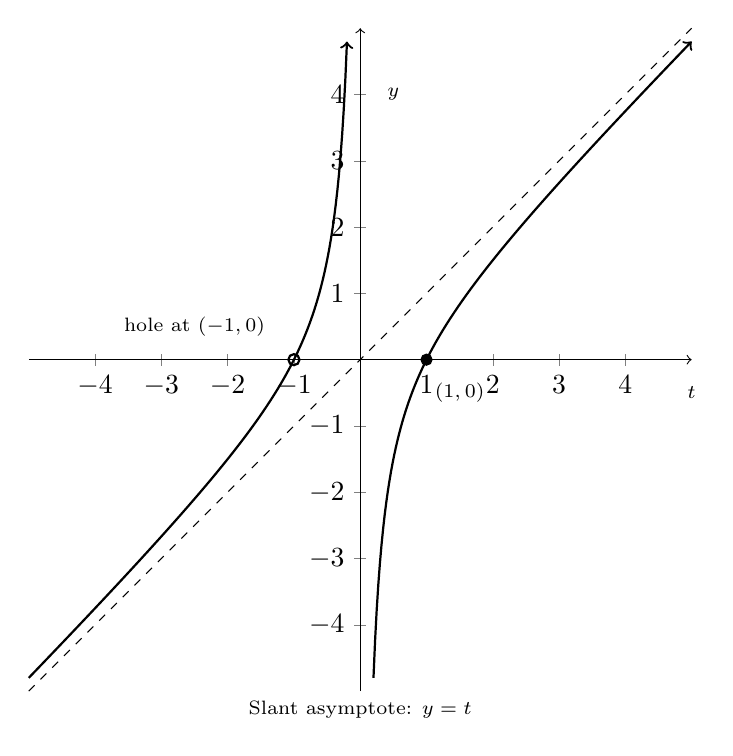
\begin{tikzpicture}
  \begin{axis}[
    axis lines=middle,
    xmin=-5, xmax=5,
    ymin=-5, ymax=5,
    xtick={-4,-3,-2,-1,1,2,3,4},
    xticklabels={$-4$,$-3$,$-2$,$-1$,$1$,$2$,$3$,$4$},
    ytick={-4,-3,-2,-1,1,2,3,4},
    yticklabels={$-4$,$-3$,$-2$,$-1$,$1$,$2$,$3$,$4$},
    axis line style={->},
    width=10cm, height=10cm,
    clip=false
  ]
    % Axis labels
    \node at (axis cs:5,-0.5) {\scriptsize $t$};
    \node at (axis cs:0.5,4) {\scriptsize $y$};

    % Slant asymptote y = t
    \addplot[dashed, domain=-5:5] {x};

    % Function pieces (avoiding discontinuity at x=0)
    \addplot[domain=-5:-0.2, samples=200, thick, ->] {x - 1/x};
    \addplot[domain=0.2:5, samples=200, thick, ->] {x - 1/x};

    % Open circle (hole) at (-1,0)
    \addplot[only marks, mark=o, mark size=2pt, thick] coordinates {(-1,0)};
    \node at (axis cs:-2.5,0.5) {\scriptsize hole at $(-1,0)$};

    % Solid point at (1,0)
    \addplot[only marks, mark=*] coordinates {(1,0)};
    \node at (axis cs:1.5,-0.5) {\scriptsize $(1,0)$};

    % Caption
    \node[below] at (rel axis cs:0.5,0) 
      {\scriptsize Slant asymptote: $y=t$};
  \end{axis}
\end{tikzpicture}
\end{problem}
 
\begin{problem}
Let $g(x) = \displaystyle \frac{x^{4} - 8x^{3} + 24x^{2} - 72x + 135}{x^{3} - 9x^{2} + 15x - 7}.\;$  With the help of your classmates:

\begin{itemize}

\item  find the $x$- and $y$- intercepts of the graph of $g$.

\item   find all of the asymptotes of the graph of $g$ and any holes in the graph, if they exist.

\item find the intervals on which the function is increasing, the intervals on which it is decreasing and the local maximums and minimums, if any exist.

\item sketch the graph of $g$, using more than one picture if necessary to show all of the important features of the graph.

\end{itemize}
\end{problem}

\begin{problem}\label{rationalneedcalcfirst}
Example \ref{carefulanalysisneeded} showed us that the six-step procedure cannot tell us everything of importance about the graph of a rational function and that sometimes there are things that are easy to miss.  Without Calculus, we may need to use graphing utilities to reveal the hidden behavior of rational functions.  Working with your classmates, use a graphing utility to examine the graphs the rational function given.  Compare and contrast their features.  Which features can the six-step process reveal and which features cannot be detected by it?   

$f(x) = \dfrac{1}{x^{2} + 1}$
\end{problem}

\begin{problem}
Example \ref{carefulanalysisneeded} showed us that the six-step procedure cannot tell us everything of importance about the graph of a rational function and that sometimes there are things that are easy to miss.  Without Calculus, we may need to use graphing utilities to reveal the hidden behavior of rational functions.  Working with your classmates, use a graphing utility to examine the graphs the rational function given.  Compare and contrast their features.  Which features can the six-step process reveal and which features cannot be detected by it?   

$f(x) = \dfrac{x}{x^{2} + 1}$ 
\end{problem}

\begin{problem}
Example \ref{carefulanalysisneeded} showed us that the six-step procedure cannot tell us everything of importance about the graph of a rational function and that sometimes there are things that are easy to miss.  Without Calculus, we may need to use graphing utilities to reveal the hidden behavior of rational functions.  Working with your classmates, use a graphing utility to examine the graphs the rational function given.  Compare and contrast their features.  Which features can the six-step process reveal and which features cannot be detected by it?  

$f(x) = \dfrac{x^{2}}{x^{2} + 1}$ 
\end{problem}

\begin{problem}\label{rationalneedcalclast}
Example \ref{carefulanalysisneeded} showed us that the six-step procedure cannot tell us everything of importance about the graph of a rational function and that sometimes there are things that are easy to miss.  Without Calculus, we may need to use graphing utilities to reveal the hidden behavior of rational functions.  Working with your classmates, use a graphing utility to examine the graphs the rational function given.  Compare and contrast their features.  Which features can the six-step process reveal and which features cannot be detected by it?   

$f(x) = \dfrac{x^{3}}{x^{2} + 1}$
\end{problem}

\end{document}


\closegraphsfile

\end{document}
